\chapter{Theory}
    \section{The Standard Model}

        \subsection{Fermions}
        Fermions are pin-$\frac{1}{2}$ particles which obey the Pauli Exclusion principle, and thus take up space and make up matter. Within the \gls{SM}, there are two types of fermions, quarks and leptons. Each of these can be broken down into three generations of particles.

        Quarks have several properties:
        \begin{itemize}
            \item Flavor - There are 6 flavors of quarks: up (u), down (d), strange (s), charm (c), bottom (b), and top (t) (from lightest to heaviest). Each particle also has a corresponding anti-particle: anti-up ($\bar{u}$), anti-down ($\bar{d}$), etc.
            \item Electric Charge - Quarks either have charge of $\frac{2}{3}$ (up, charm, top) or $-\frac{1}{3}$ (down, strange, bottom), while anti-quarks have the opposite charge. 
            \item Color Charge - Each quark has a degree of freedom known as color charge, which can be `red', `blue', or `green', as well as a corresponding anti-color. Bound states require a colorless configuration, which may be achieved either through a color-anticolor combination known as mesons, or a (anti)-RGB triplet known as (anti)-baryons.
        \end{itemize}

        % TODO: leptons

        Generally, the wave function of a fermion is given by $\psi(x)$, and is a spinor of four components. The motion is described by the relativistic version of the Schr{\"o}dinger equation known as the Dirac equation, given as

        \begin{equation}
            (i\gamma'^{\mu}\partial_{\mu}-m)\Psi' = 0
        \end{equation}


        \subsection{Bosons}


%%%%%% Forces %%%%%%%%        
\subsection{Forces}
In nature, there are four fundamental forces describing interactions: the strong nuclear force, the weak nuclear force, the electromagnetic force, and the gravitational force. The \gls{SM} models the former three of these forces\footnote{The gravitational force is not modeled by the \gls{SM}. It has relative strength of $10^{-37}$ at $\unit{1}{fm}$. In theories of quantum gravity, it is mediated by the ``graviton'' ($G$), a massless spin-2 particle.}, describing each via a \gls{QFT} corresponding to the exchange of a gauge boson. A broad summary of the forces and their associated \glspl{QFT} can be found in \ref{tab:forces}.

\begin{table}[!ht]
    \begin{tabular}{l|l|l|l}
    Force & Field Theory & Boson & Relative Strength      \\ \hline
    Strong Nuclear   & Quantum Chromodynamics  & Gluon ($g$) & $1$ \\
    Electromagnetism & Quantum Electrodynamics & Photon ($\gamma$) & $10^{-3}$ \\
    Weak Nuclear     & Quantum Flavordynamics  & $W^{\pm}$, $Z$ & $10^{-8}$
    \end{tabular}
    \caption{List of forces described by the \gls{SM}, as well as their associated field theory and gauge boson mediator. Relative strength is an order of magnitude estimate at a distance of $\unit{1}{fm}$.}
    \label{tab:forces}
\end{table}

\subsubsection{Electromagnetic Force}
The electromagnetic interaction corresponds to a \gls{QFT} known as \gls{QED}. In \gls{QED}, the fermonic spinor field, $\Psi$, carries electric charge proportional to the charge of the electron $Qe$. For electrons and positrons, Q takes the value -1, and for quarks it takes either +2/3 ($u$,$c$,$t$) or -1/3($d$,$s$,$b$). The interaction Lagrangian density for a fermion with this charge and electromagnetic field is

\begin{equation}
    \mathcal{L}_{int} = -eQ\bar{\Psi}\gamma^{\mu}\Psi A_{\mu}
\end{equation}

For electromagnetic field $A^{\mu}$.

\subsubsection{Strong Nuclear Force}

The strong nuclear force is the strongest force, but acts only at a short range. The mediator of the strong interaction is a massless spin-1 gauge boson called the gluon.

\subsubsection{Weak Nuclear Force}


%%%%%% Di-Higgs %%%%%%%%                
\section{The Higgs Field and Higgs Boson}

The minimal Higgs model has two complex scalar fields, which are placed in a weak isospin doublet

\begin{equation}
\phi = \begin{pmatrix} \phi^+ \\ \phi^0 \end{pmatrix}
    = \frac{1}{\sqrt{2}}\begin{pmatrix}
        \phi_1 + i\phi_2 \\ \phi_3 + i\phi_4
    \end{pmatrix}
\end{equation}

With corresponding Lagrangian

\begin{equation} \label{higgs-lagrangian}
    \mathcal{L} = (\partial_{\mu}\phi)^\dagger (\partial^{\mu}\phi) - V(\phi)\\
\end{equation}

And potential,

\begin{equation} \label{higgs-potential}
    V(\phi) = \mu^2\phi^\dagger \phi - \lambda(\phi^\dagger \phi)^2
\end{equation}

The minima of this potential is known as the vacuum state, and for this minima to be finite, $\lambda$ must be greater than 0. For $\mu^2 >0$, the minima is located at 0, however, for $\mu^2<0$, the potential has minima at:

\begin{equation}
    \phi^\dagger \phi = \frac{1}{2}(\phi_{1}^{2}+\phi_{2}^{2}+\phi_{3}^{2}+\phi_{4}^{2}) = \frac{v^2}{2} = -\frac{\mu^2}{2\lambda}
\end{equation}

This value is known as the \glsfirst{vev}. When $\mu^2 < 0$, this value is non-zero, and due to symmetry has two degenerate states. By choosing state, the Lagrangian symmetry is broken, known as spontaneous symmetry breaking.

\begin{figure}[!ht]
    \centering
    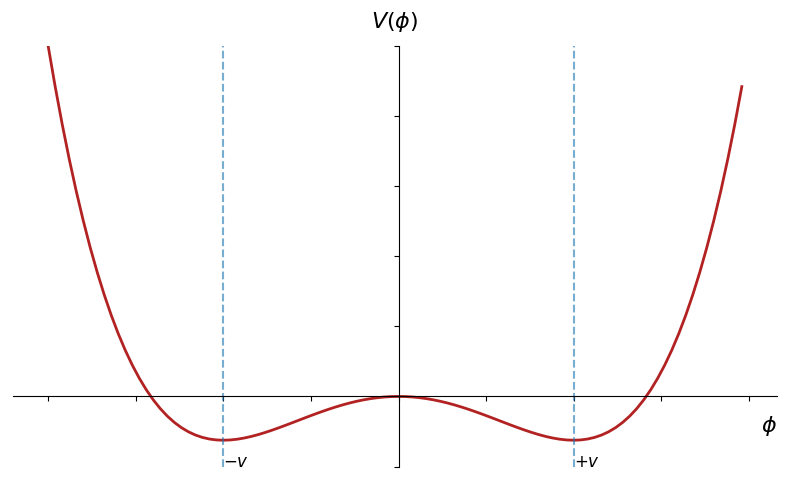
\includegraphics[width=\textwidth]{chapters/chapter1_theory/images/higgs-2d-vev.png}
    \caption{The one-dimensional Higgs potential where $\mu^2 <0$. The minima of this curve, known as the Higgs \gls{vev}, is indicated.}
    \label{fig:higgs-potential}
\end{figure}


\begin{equation} \label{higgs-lagrangian}
    \begin{aligned}
        \mathcal{L} &= \frac{1}{2}(\partial_{\mu}\phi)(\partial^{\mu}\phi) - V(\phi)\\
        &= \frac{1}{2}(\partial_{\mu}\phi)(\partial^{\mu}\phi) - \frac{1}{2}\mu^2\phi^2 - \frac{1}{2}\lambda\phi^4
    \end{aligned}
\end{equation}



%%%%%% Di-Higgs %%%%%%%%                
\section{Di-Higgs Production}
The analysis presented in this thesis searches for di-Higgs production - processes that pair produce Higgs bosons. This process is rare, the total cross-section being {\color{red} 30} fb at 13 TeV center-of-mass energy.

\subsection{Production in the Standard Model}
In the standard model, several production modes pair produce Higgs bosons. Gluon-gluon Fusion (ggF) is the most dominant with a cross-section of {\color{red} 33} fb, accounting for {\color{red} 89\%} of di-Higgs production. The next most dominant is Vector Boson Fusion. The remaining production modes, VHH, ttHH, and bbHH collectively comprise less than 5\% of di-Higgs production, and have a cross-section too small to make a meaningful contribution to the proposed analysis.

\subsubsection{Gluon-Gluon Fusion}
        \subsubsection{Vector Boson Fusion}
    \subsection{Production Beyond the Standard Model}
        \subsubsection{Resonant BSM Production}
        \subsubsection{Non-Resonant BSM Production}

